\subsubsection{Flujos de gestión}

Los flujos de gestión definen el ciclo de vida de los objetos del Directorio en la aplicación, asegurando que las operaciones realizadas por los administradores se sincronicen correctamente con el AD. Estas operaciones incluyen la creación, lectura, actualización y eliminación de objetos.

\textbf{Creación de objetos}

Cuando un nuevo objeto, como un usuario o grupo, es creado desde la aplicación, este es registrado en el AD mediante una operación add (\autoref{fig:ldap-add-operation}). El cliente LDAP, ldapts, se utiliza para establecer una conexión segura y confiable con el servidor del AD, donde se envían los atributos requeridos para el nuevo objeto. A lo largo del proceso, se validan los datos, y cualquier error encontrado es notificado al usuario tal y como se muestra en la \autoref{fig:activity-diagram-create-user}.

\begin{figure}[h]
    \centering
    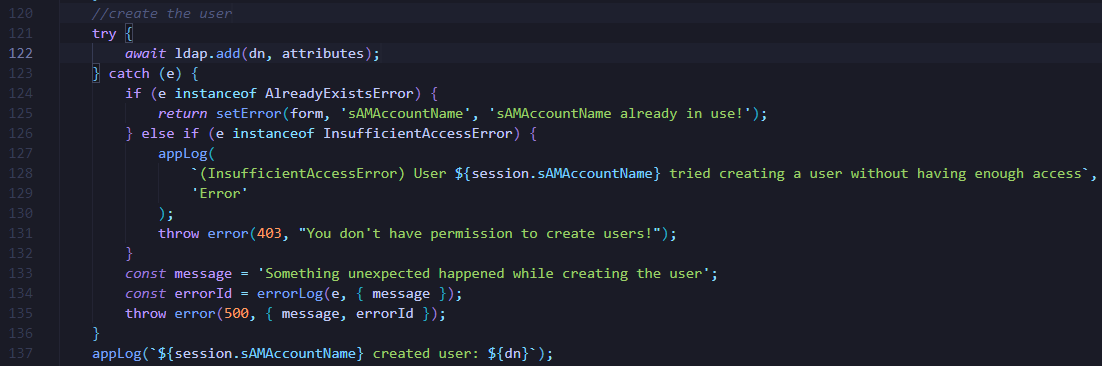
\includegraphics[width=\linewidth]{images/code/ldap-add-operation.png}
    \caption{Uso de la operacion \textit{add} con el cliente LDAP}
    \label{fig:ldap-add-operation}
\end{figure}

\textbf{Lectura de objetos}

La lectura de objetos permite a los administradores consultar los detalles de los usuarios, grupos y otros elementos en el AD. Esta operación se realiza mediante el cliente LDAP utilizando la función de búsqueda, filtrando los resultados con base en los parámetros establecidos. Los administradores pueden visualizar los detalles de los objetos, incluidas sus propiedades y relaciones con otros objetos. En la \autoref{fig:get-all-users} se muestra la función getAllUsers donde se utiliza la operación search aplicando determinados filtros para obtener las entradas del directorio que sean del esquema usuario.

\begin{figure}[h]
    \centering
    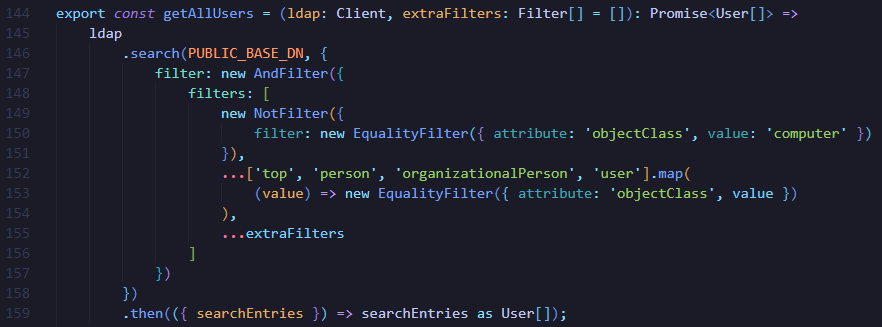
\includegraphics[width=\linewidth]{images/code/getAllUsers.png}
    \caption{Uso de la operación \textit{search} del cliente LDAP para listar usuarios}
    \label{fig:get-all-users}
\end{figure}

\textbf{Actualización de objetos}

La actualización de objetos en el AD se gestiona a través de operaciones \textbf{modify} o \textbf{replace}. La aplicación permite a los administradores modificar los atributos de los objetos, como los datos personales de un usuario o la membresía de un grupo. Una vez validados los cambios, estos se aplican directamente al AD, asegurando que la información sea precisa y esté actualizada. En la \autoref{fig:flow-diagram-update-group} se detalla el flujo de actualización de un grupo.

\textbf{Eliminación de objetos}

Finalmente, la eliminación de objetos se maneja mediante una operación delete. Los administradores pueden eliminar usuarios, grupos o unidades organizativas, y el cambio se refleja de inmediato en el AD. Antes de la eliminación, se realizan verificaciones adicionales para evitar la pérdida de información importante o la eliminación accidental de objetos clave. En la \autoref{fig:activity-diagram-delete-ou} se muestra el diagrama de actividades para el proceso de eliminar una Unidad Organizacional.
